\par
\section{Driver programs for the {\tt InpMtx} object}
\label{section:InpMtx:drivers}
\par
This section contains brief descriptions of the driver programs.
\par
%=======================================================================
\begin{enumerate}
%-----------------------------------------------------------------------
\item
\begin{verbatim}
testIO msglvl msgFile inFile outFile
\end{verbatim}
This driver program reads and write {\tt InpMtx} files, useful for
converting formatted files to binary files and vice versa.
One can also read in a {\tt InpMtx} file and print out just the 
header information (see the {\tt InpMtx\_writeStats()} method).
\par
\begin{itemize}
\item
The {\tt msglvl} parameter determines the amount of output ---
taking {\tt msglvl >= 3} means the {\tt InpMtx} object is written
to the message file.
\item
The {\tt msgFile} parameter determines the message file --- if {\tt
msgFile} is {\tt stdout}, then the message file is {\it stdout},
otherwise a file is opened with {\it append} status to receive any
output data.
\item
The {\tt inFile} parameter is the input file for the {\tt InpMtx}
object. It must be of the form {\tt *.inpmtxf} or {\tt *.inpmtxb}.
The {\tt InpMtx} object is read from the file via the
{\tt InpMtx\_readFromFile()} method.
\item
The {\tt outFile} parameter is the output file for the {\tt InpMtx}
object. 
If {\tt outFile} is {\tt none} then the {\tt InpMtx} object is not
written to a file. 
Otherwise, the {\tt InpMtx\_writeToFile()} method is called to write
the object to 
a formatted file (if {\tt outFile} is of the form {\tt *.inpmtxf}),
or
a binary file (if {\tt outFile} is of the form {\tt *.inpmtxb}).
\end{itemize}
%-----------------------------------------------------------------------
\item
\begin{verbatim}
testFullAdj msglvl msgFile nvtx nent seed
\end{verbatim}
This driver program tests the {\tt InpMtx\_fullAdjacency()} method.
If first generates a {\tt InpMtx} object filled with
random entries of a matrix $A$ and then constructs an {\tt IVL}
object that contains the full adjacency structure of $A + A^T$,
diagonal edges included.
\par
\begin{itemize}
\item
The {\tt msglvl} parameter determines the amount of output ---
taking {\tt msglvl >= 3} means the {\tt InpMtx} object is written
to the message file.
\item
The {\tt msgFile} parameter determines the message file --- if {\tt
msgFile} is {\tt stdout}, then the message file is {\it stdout},
otherwise a file is opened with {\it append} status to receive any
output data.
\item
The {\tt nvtx} parameter is the number of rows and columns in $A$.
\item
The {\tt nent} parameter is an upper bound on the number of entries
in $A$. (Since the locations of the entries are generated via
random numbers, there may be duplicate entries.) 
\item
The {\tt seed} parameter is random number seed.
\end{itemize}
%-----------------------------------------------------------------------
\item
\begin{verbatim}
testFullAdj2 msglvl msgFile nvtx nentA nentB seed
\end{verbatim}
This driver program tests the {\tt InpMtx\_fullAdjacency2()} method.
If first generates two {\tt InpMtx} object filled with
random entries --- one for a matrix $A$ and one for a matrix $B$.
It then constructs an {\tt IVL}
object that contains the full adjacency structure of $(A+B) + (A+B)^T$,
diagonal edges included.
\par
\begin{itemize}
\item
The {\tt msglvl} parameter determines the amount of output ---
taking {\tt msglvl >= 3} means the {\tt InpMtx} object is written
to the message file.
\item
The {\tt msgFile} parameter determines the message file --- if {\tt
msgFile} is {\tt stdout}, then the message file is {\it stdout},
otherwise a file is opened with {\it append} status to receive any
output data.
\item
The {\tt nvtx} parameter is the number of rows and columns in $A$.
\item
The {\tt nentA} parameter is an upper bound on the number of entries
in $A$. (Since the locations of the entries are generated via
random numbers, there may be duplicate entries.) 
\item
The {\tt nentB} parameter is an upper bound on the number of entries
in $B$. (Since the locations of the entries are generated via
random numbers, there may be duplicate entries.) 
\item
The {\tt seed} parameter is random number seed.
\end{itemize}
%-----------------------------------------------------------------------
\item
\begin{verbatim}
createGraph msglvl msgFile inFile outFile
\end{verbatim}
This driver program reads in {\tt InpMtx} object from the file
{\tt inFile} that holds a matrix $A$.
It then creates a {\tt Graph} object for $B = A + A^T$
and writes it to the file {\tt outFile}.
Recall, a {\tt Graph} object must be symmetric, so if the {\tt
InpMtx} object only holds the lower or upper triangular part 
of the matrix, the other portion will be added.
Also, a {\tt Graph} object has edges of the form {\tt (v,v)},
and if these entries are missing from the {\tt InpMtx} object,
they will be added.
\par
\begin{itemize}
\item
The {\tt msglvl} parameter determines the amount of output ---
taking {\tt msglvl >= 3} means the {\tt InpMtx} object is written
to the message file.
\item
The {\tt msgFile} parameter determines the message file --- if {\tt
msgFile} is {\tt stdout}, then the message file is {\it stdout},
otherwise a file is opened with {\it append} status to receive any
output data.
\item
The {\tt inFile} parameter is the input file for the {\tt InpMtx}
object. It must be of the form {\tt *.inpmtxf} or {\tt *.inpmtxb}.
The {\tt InpMtx} object is read from the file via the
{\tt InpMtx\_readFromFile()} method.
\item
The {\tt outFile} parameter is the output file for the {\tt InpMtx}
object. 
If {\tt outFile} is {\tt none} then the {\tt InpMtx} object is not
written to a file. 
Otherwise, the {\tt InpMtx\_writeToFile()} method is called to write
the object to 
a formatted file (if {\tt outFile} is of the form {\tt *.inpmtxf}),
or
a binary file (if {\tt outFile} is of the form {\tt *.inpmtxb}).
\end{itemize}
%-----------------------------------------------------------------------
\item
\begin{verbatim}
createGraphForATA msglvl msgFile inFile outFile
\end{verbatim}
This driver program reads in {\tt InpMtx} object from the file
{\tt inFile} that holds a matrix $A$.
It then creates a {\tt Graph} object for $B = A^TA$
and writes it to the file {\tt outFile}.
\par
\begin{itemize}
\item
The {\tt msglvl} parameter determines the amount of output ---
taking {\tt msglvl >= 3} means the {\tt InpMtx} object is written
to the message file.
\item
The {\tt msgFile} parameter determines the message file --- if {\tt
msgFile} is {\tt stdout}, then the message file is {\it stdout},
otherwise a file is opened with {\it append} status to receive any
output data.
\item
The {\tt inFile} parameter is the input file for the {\tt InpMtx}
object. It must be of the form {\tt *.inpmtxf} or {\tt *.inpmtxb}.
The {\tt InpMtx} object is read from the file via the
{\tt InpMtx\_readFromFile()} method.
\item
The {\tt outFile} parameter is the output file for the {\tt InpMtx}
object. 
If {\tt outFile} is {\tt none} then the {\tt InpMtx} object is not
written to a file. 
Otherwise, the {\tt InpMtx\_writeToFile()} method is called to write
the object to 
a formatted file (if {\tt outFile} is of the form {\tt *.inpmtxf}),
or
a binary file (if {\tt outFile} is of the form {\tt *.inpmtxb}).
\end{itemize}
%-----------------------------------------------------------------------
\item
\begin{verbatim}
adjToGraph msglvl msgFile inAdjacencyFile outGraphFile flag
\end{verbatim}
This driver program was used to generate a {\tt type 0} {\tt Graph} 
object (unit weight vertices and edges) from
a file that contained the adjacency structure of a matrix in the
following form.
\begin{verbatim}
      nvtx nadj
      offsets[nvtx+1]
      indices[nadj]
\end{verbatim}
There are {\tt nvtx} vertices in the graph and the adjacency vector
has {\tt nadj} entries.
It was not known whether the adjacency structure contained 
{\tt (v,v)} entries or if it was only the upper or lower triangle.
Our {\tt Graph} object is symmetric with loops, i.e.,
{\tt (u,v)} is present if and only if {\tt (v,u)} is present,
and {\tt (v,v)} is present.
\par
This program reads in the adjacency structure, decrements the
offsets and indices by one if specified by the flag parameter
(our application came from a Fortran code with 1-indexing),
then loads the entries into a {\tt InpMtx} object where they are
assembled and sorted by rows.
The $(v,v)$ entries are loaded, and each vector of the adjacency
structure is loaded as both a column and as a row, so in effect we
are constructing the graph of $(A+A^T)$.
Recall, multiple entries are collapsed during the sort and merge
step.
\par
A {\tt Graph} object is then created using the {\tt
Graph\_fillFromOffsets()} method using the vectors in the {\tt
InpMtx} object.
The {\tt Graph} object is then optionally written to a file.
\par
\begin{itemize}
\item
The {\tt msglvl} parameter determines the amount of output ---
taking {\tt msglvl >= 3} means the {\tt InpMtx} object is written
to the message file.
\item
The {\tt msgFile} parameter determines the message file --- if {\tt
msgFile} is {\tt stdout}, then the message file is {\it stdout},
otherwise a file is opened with {\it append} status to receive any
output data.
\item
The {\tt inAdjacencyFile} parameter is the input file for the 
adjacency structure as defined above.
It must be a formatted file.
\item
The {\tt outGraphFile} parameter is the output file for the 
{\tt Graph} object. 
If {\tt outGraphFile} is {\tt none} then the {\tt Graph} object is not
written to a file. 
Otherwise, the {\tt Graph\_writeToFile()} method is called to write
the object to 
a formatted file (if {\tt outGraphFile} is of the form 
{\tt *.graphf}),
or
a binary file (if {\tt outGraphFile} is of the form {\tt *.graphb}).
\item
The {\tt flag} parameter is used to specify whether the offsets
and indices are 0-indexed (as in C) or 1-indexed (as in Fortran).
If they are 1-indexed, the offsets and indices are decremented
prior to loading into the {\tt InpMtx} object.
\end{itemize}
%-----------------------------------------------------------------------
\item
\begin{verbatim}
weightedAdjToGraph msglvl msgFile inAdjacencyFile outGraphFile flag
\end{verbatim}
This driver program was used to generate a {\tt type 1} {\tt Graph} 
object (weighted vertices, unit weight edges) from
a file that contained the adjacency structure of a matrix in the
following form.
\begin{verbatim}
      nvtx nadj
      vwghts[nvtx]
      offsets[nvtx+1]
      indices[nadj]
\end{verbatim}
There are {\tt nvtx} vertices in the graph and the adjacency vector
has {\tt nadj} entries.
It was not known whether the adjacency structure contained 
{\tt (v,v)} entries or if it was only the upper or lower triangle.
Our {\tt Graph} object is symmetric with loops, i.e.,
{\tt (u,v)} is present if and only if {\tt (v,u)} is present,
and {\tt (v,v)} is present.
\par
This program reads in the adjacency structure, decrements the
offsets and indices by one if specified by the flag parameter
(our application came from a Fortran code with 1-indexing),
then loads the entries into a {\tt InpMtx} object where they are
assembled and sorted by rows.
The $(v,v)$ entries are loaded, and each vector of the adjacency
structure is loaded as both a column and as a row, so in effect we
are constructing the graph of $(A+A^T)$.
Recall, multiple entries are collapsed during the sort and merge
step.
\par
A {\tt Graph} object is then created using the {\tt
Graph\_fillFromOffsets()} method using the vectors in the {\tt
InpMtx} object.
The {\tt Graph} object is then optionally written to a file.
\par
\begin{itemize}
\item
The {\tt msglvl} parameter determines the amount of output ---
taking {\tt msglvl >= 3} means the {\tt InpMtx} object is written
to the message file.
\item
The {\tt msgFile} parameter determines the message file --- if {\tt
msgFile} is {\tt stdout}, then the message file is {\it stdout},
otherwise a file is opened with {\it append} status to receive any
output data.
\item
The {\tt inAdjacencyFile} parameter is the input file for the 
adjacency structure as defined above.
It must be a formatted file.
\item
The {\tt outGraphFile} parameter is the output file for the 
{\tt Graph} object. 
If {\tt outGraphFile} is {\tt none} then the {\tt Graph} object is not
written to a file. 
Otherwise, the {\tt Graph\_writeToFile()} method is called to write
the object to 
a formatted file (if {\tt outGraphFile} is of the form 
{\tt *.graphf}),
or
a binary file (if {\tt outGraphFile} is of the form {\tt *.graphb}).
\item
The {\tt flag} parameter is used to specify whether the offsets
and indices are 0-indexed (as in C) or 1-indexed (as in Fortran).
If they are 1-indexed, the offsets and indices are decremented
prior to loading into the {\tt InpMtx} object.
\end{itemize}
%-----------------------------------------------------------------------
\item
\begin{verbatim}
testR2D msglvl msgFile EGraphFile CoordsFile coordType seed outInpMtxFile
\end{verbatim}
This driver program reads in an {\tt EGraph} element graph and a
{\tt Coords} grid point coordinate object for one of the {\tt R2D*}
randomly triangulated 2-D grids.
It then generates the finite element matrices for each of the
triangular elements and assembles the matrices into a {\tt InpMtx}
object, which is then optionally written out to a file.
A matrix-vector product is computed using the unassembled matrix
and the assembled matrix and compared to detect errors. 
The {\tt InpMtx} object is then permuted and a matrix-vector
multiply again computed and checked for errors.
\begin{itemize}
\item
The {\tt msglvl} parameter determines the amount of output ---
taking {\tt msglvl >= 3} means that all objects are written
to the message file.
\item
The {\tt msgFile} parameter determines the message file --- if {\tt
msgFile} is {\tt stdout}, then the message file is {\it stdout},
otherwise a file is opened with {\it append} status to receive any
message data.
\item
The {\tt EGraphFile} is the file that holds the {\tt EGraph}
object --- must be of the form {\tt *.egraphf} or {\tt *.egraphb}.
\item
The {\tt CoordsFile} is the file that holds the {\tt Coords}
object --- must be of the form {\tt *.coordsf} or {\tt *.coordsb}.
\item
The {\tt coordType} determines the coordinate type for the {\tt
InpMtx} object.
\begin{itemize}
\item {\tt 1} --- storage of entries by rows
\item {\tt 2} --- storage of entries by columns
\item {\tt 3} --- storage of entries by chevrons
\end{itemize}
\item
The {\tt seed} parameter is used as a random number seed to
determine the row and column permutations for the matrix-vector
multiply.
\item
The {\tt outInpMtxFile} parameter is the output file for the 
{\tt InpMtx} object. 
If {\tt outInpMtxFile} is {\tt none} then the {\tt InpMtx} object 
is not written to a file. 
Otherwise, the {\tt InpMtx\_writeToFile()} method is called to write
the object to 
a formatted file (if {\tt outInpMtxFile} 
is of the form {\tt *.inpmtxf}), or
a binary file (if {\tt outInpMtxFile} is of the form {\tt *.inpmtxb}).
\end{itemize}
%-----------------------------------------------------------------------
\item
\begin{verbatim}
readAIJ msglvl msgFile inputFile outInpMtxFile flag
\end{verbatim}
This driver program reads $(i,j,a_{i,j})$ triples from a file,
loads them into a {\tt InpMtx} object,
and optionally writes the object out to a file.
The input file has the form:
\begin{itemize}
\item
The {\tt msglvl} parameter determines the amount of output ---
taking {\tt msglvl >= 3} means that all objects are written
to the message file.
\item
The {\tt msgFile} parameter determines the message file --- if {\tt
msgFile} is {\tt stdout}, then the message file is {\it stdout},
otherwise a file is opened with {\it append} status to receive any
message data.
\item
The {\tt inputFile} is the file that holds the triples.
It has the following form.
\begin{verbatim}
nrow ncol nentries
irow jcol value
 ...
irow jcol value
\end{verbatim}
Note, {\tt nrow} and {\tt ncol} are not used by the {\tt InpMtx}
object --- each (irow, jcol, value) triple is loaded.
\item
The {\tt outInpMtxFile} parameter is the output file for the 
{\tt InpMtx} object. 
If {\tt outInpMtxFile} is {\tt none} then the {\tt InpMtx} object 
is not written to a file. 
Otherwise, the {\tt InpMtx\_writeToFile()} method is called to write
the object to 
a formatted file (if {\tt outInpMtxFile} 
is of the form {\tt *.inpmtxf}), or
a binary file (if {\tt outInpMtxFile} is of the form {\tt *.inpmtxb}).
\item
The {\tt flag} parameter is used to specify whether the 
indices are 0-indexed (as in C) or 1-indexed (as in Fortran).
If they are 1-indexed, the indices are decremented
prior to loading into the {\tt InpMtx} object.
\end{itemize}
%-----------------------------------------------------------------------
\item
\begin{verbatim}
getProfile msglvl msgFile inInpMtxFile npts tausmall taubig
\end{verbatim}
This driver program produces a profile of the magnitudes 
of the matrix entries in a format that is suitable for plotting
by Matlab.
The {\tt npts} parameter specifies how many points to be used
in the profile plot.
The message file will contain line of the form.
\begin{verbatim}
    data = [ ...
        x1    y1
        ...
        xnpts ynpts ] ;
\end{verbatim}
which can be used to generate the following matlab plot.
An example is given below for the {\sc bcsstk23} matrix, where
{\tt npts = 200}, {\tt tausmall = 1.e-10} and
{\tt taubig = 1.e100}.
\begin{center}
\makebox{
% \psfig{file=BCSSTK23.eps,width=3.0in,height=2.40in}
\psfig{file=../../InpMtx/doc/BCSSTK23.eps,width=3.0in,height=2.40in}
}
\end{center}
The number of entries that are zero,
the number whose magnitude is less than {\tt tausmall},
and the number whose magnitude is larger than {\tt taubig}
are printed to {\tt msgFile}.
\par
\begin{itemize}
\item
The {\tt msglvl} parameter determines the amount of output ---
taking {\tt msglvl >= 3} means the {\tt InpMtx} object is written
to the message file.
\item
The {\tt msgFile} parameter determines the message file --- if {\tt
msgFile} is {\tt stdout}, then the message file is {\it stdout},
otherwise a file is opened with {\it append} status to receive any
output data.
\item
The {\tt inInpMtxFile} parameter is the input file for 
the {\tt InpMtx} object that holds the matrix.
It must be of the form {\tt *.inpmtxf} or {\tt *.inpmtxb}.
The {\tt InpMtx} object is read from the file via the
{\tt InpMtx\_readFromFile()} method.
\item
The {\tt npts} parameter determines the number of points to use in
the plot.
\item
The {\tt tausmall} parameter is a lower cutoff for putting entries
in the profile plot.
\item
The {\tt taubig} parameter is an upper cutoff for putting entries
in the profile plot.
\end{itemize}
%-----------------------------------------------------------------------
\item
\begin{verbatim}
mkNaturalFactorMtx msglvl msgFile n1 n2 n3 seed outFile 
\end{verbatim}
This driver program generates rectangular matrix that would arise
from a natural factor representation of the Laplacian operator on a
regular grid.
If {\tt n3 = 1}, we have a ${\tt n1} \times {\tt n2}$ grid.
There are {\tt (n1-1)*(n2-1)} elements and each element gives rise
to four equations, so the resulting matrix has
{\tt 4(n1-1)*(n2-1)} rows and {\tt n1*n2} columns.
If {\tt n3 > 1}, 
we have a ${\tt n1} \times {\tt n2} \times {\tt n3}$ grid.
There are {\tt (n1-1)*(n2-1)*(n3-1)} elements 
and each element gives rise
to eight equations, so the resulting matrix has
{\tt 8(n1-1)*(n2-1)*(n3-1)} rows and {\tt n1*n2*n3} columns.
\par
\begin{itemize}
\item
The {\tt msglvl} parameter determines the amount of output ---
taking {\tt msglvl >= 3} means the {\tt InpMtx} object is written
to the message file.
\item
The {\tt msgFile} parameter determines the message file --- if {\tt
msgFile} is {\tt stdout}, then the message file is {\it stdout},
otherwise a file is opened with {\it append} status to receive any
output data.
\item
{\tt n1} is the number of points in the first direction.
\item
{\tt n2} is the number of points in the second direction.
\item
{\tt n3} is the number of points in the third direction.
\item
The {\tt seed} parameter is a random number seed used to fill the
matrix entries with random numbers.
\item
The {\tt outFile} parameter is the output file for 
the {\tt InpMtx} object that holds the matrix.
It must be of the form {\tt *.inpmtxf} or {\tt *.inpmtxb}.
The {\tt InpMtx} object is written to the file via the
{\tt InpMtx\_writeToFile()} method.
\end{itemize}
%-----------------------------------------------------------------------
\item
\begin{verbatim}
testMMM msglvl msgFile dataType symflag coordType transpose
        nrow ncol nitem nrhs seed alphaReal alphaImag
\end{verbatim}
This driver program tests the matrix-matrix multiply methods.
This driver program generates $A$, a 
${\tt nrow} \times {\tt ncol}$
matrix using {\tt nitem} input entries, $X$ and $Y$,
${\tt nrow} \times {\tt nrhs}$ matrices,
and all are filled with random numbers.
It then computes 
$Y := Y + \alpha A X$, 
$Y := Y + \alpha A^T X$ or
$Y := Y + \alpha A^H X$.
The program's output is a file which when sent into Matlab,
outputs the error in the computation.
\par
\begin{itemize}
\item
The {\tt msglvl} parameter determines the amount of output ---
taking {\tt msglvl >= 3} means the {\tt InpMtx} object is written
to the message file.
\item
The {\tt msgFile} parameter determines the message file --- if {\tt
msgFile} is {\tt stdout}, then the message file is {\it stdout},
otherwise a file is opened with {\it append} status to receive any
output data.
\item
{\tt dataType} is the type of entries,
{\tt 0} for real, {\tt 1} for complex.
\item
{\tt symflag} is the symmetry flag, {\tt 0} for symmetric, 
{\tt 1} for Hermitian, {\tt 2} for nonsymmetric.
\item
{\tt coordType} is the storage mode for the entries, 
{\tt 1} for by rows, {\tt 2} for by columns, 
{\tt 3} for by chevrons. 
\item
{\tt transpose} determines the equation,
{\tt 0} for $Y := Y + \alpha A X$, 
{\tt 1} for $Y := Y + \alpha A^H X$ or
{\tt 2} for $Y := Y + \alpha A^T X$.
\item
{\tt nrowA} is the number of rows in $A$
\item
{\tt ncolA} is the number of columns in $A$
\item
{\tt nitem} is the number of matrix entries that are 
assembled into the matrix.
\item
{\tt nrhs} is the number of columns in $X$ and $Y$.
\item
The {\tt seed} parameter is a random number seed used to fill the
matrix entries with random numbers.
\item
{\tt alphaReal} and {\tt alphaImag} form the scalar in the multiply.
\end{itemize}
%-----------------------------------------------------------------------
\item
\begin{verbatim}
testGMMM msglvl msgFile dataType symflag coordType transpose
         nrow ncol nitem nrhs seed alphaReal alphaImag betaReal betaImag
\end{verbatim}
This driver program 
tests the generalized matrix-matrix multiply methods.
It generates $A$, a 
${\tt nrow} \times {\tt ncol}$
matrix using {\tt nitem} input entries, $X$ and $Y$,
${\tt nrow} \times {\tt nrhs}$ matrices,
and all are filled with random numbers.
It then computes 
$Y := \beta Y + \alpha A X$, 
$Y := \beta Y + \alpha A^T X$ or
$Y := \beta Y + \alpha A^H X$.
The program's output is a file which when sent into Matlab,
outputs the error in the computation.
\par
\begin{itemize}
\item
The {\tt msglvl} parameter determines the amount of output ---
taking {\tt msglvl >= 3} means the {\tt InpMtx} object is written
to the message file.
\item
The {\tt msgFile} parameter determines the message file --- if {\tt
msgFile} is {\tt stdout}, then the message file is {\it stdout},
otherwise a file is opened with {\it append} status to receive any
output data.
\item
{\tt dataType} is the type of entries,
{\tt 0} for real, {\tt 1} for complex.
\item
{\tt symflag} is the symmetry flag, {\tt 0} for symmetric, 
{\tt 1} for Hermitian, {\tt 2} for nonsymmetric.
\item
{\tt coordType} is the storage mode for the entries, 
{\tt 1} for by rows, {\tt 2} for by columns, 
{\tt 3} for by chevrons. 
\item
{\tt transpose} determines the equation,
{\tt 0} for $Y := \beta Y + \alpha A X$, 
{\tt 1} for $Y := \beta Y + \alpha A^H X$ or
{\tt 2} for $Y := \beta Y + \alpha A^T X$.
\item
{\tt nrowA} is the number of rows in $A$
\item
{\tt ncolA} is the number of columns in $A$
\item
{\tt nitem} is the number of matrix entries that are 
assembled into the matrix.
\item
{\tt nrhs} is the number of columns in $X$ and $Y$.
\item
The {\tt seed} parameter is a random number seed used to fill the
matrix entries with random numbers.
\item
{\tt alphaReal} and {\tt alphaImag} 
form the $\alpha$ scalar in the multiply.
\item
{\tt betaReal} and {\tt betaImag} 
form the $\beta$ scalar in the multiply.
\end{itemize}
%-----------------------------------------------------------------------
\item
\begin{verbatim}
testGMVM msglvl msgFile dataType symflag coordType transpose
         nrow ncol nitem seed alphaReal alphaImag betaReal betaImag
\end{verbatim}
This driver program 
tests the generalized matrix-vector multiply methods.
It generates $A$, a 
${\tt nrow} \times {\tt ncol}$
matrix using {\tt nitem} input entries, 
$x$ and $y$,
and fills the matrices with random numbers.
It then computes 
$y := \beta y + \alpha A x$, 
$y := \beta y + \alpha A^T x$ or
$y := \beta y + \alpha A^H x$.
The program's output is a file which when sent into Matlab,
outputs the error in the computation.
\par
\begin{itemize}
\item
The {\tt msglvl} parameter determines the amount of output ---
taking {\tt msglvl >= 3} means the {\tt InpMtx} object is written
to the message file.
\item
The {\tt msgFile} parameter determines the message file --- if {\tt
msgFile} is {\tt stdout}, then the message file is {\it stdout},
otherwise a file is opened with {\it append} status to receive any
output data.
\item
{\tt dataType} is the type of entries,
{\tt 0} for real, {\tt 1} for complex.
\item
{\tt symflag} is the symmetry flag, {\tt 0} for symmetric, 
{\tt 1} for Hermitian, {\tt 2} for nonsymmetric.
\item
{\tt coordType} is the storage mode for the entries, 
{\tt 1} for by rows, {\tt 2} for by columns, 
{\tt 3} for by chevrons. 
\item
{\tt transpose} determines the equation,
{\tt 0} for $y := \beta y + \alpha A x$, 
{\tt 1} for $y := \beta y + \alpha A^T x$ or
{\tt 2} for $y := \beta y + \alpha A^H x$.
\item
{\tt nrowA} is the number of rows in $A$
\item
{\tt ncolA} is the number of columns in $A$
\item
{\tt nitem} is the number of matrix entries that are 
assembled into the matrix.
\item
The {\tt seed} parameter is a random number seed used to fill the
matrix entries with random numbers.
\item
{\tt alphaReal} and {\tt alphaImag} 
form the $\alpha$ scalar in the multiply.
\item
{\tt betaReal} and {\tt betaImag} 
form the $\beta$ scalar in the multiply.
\end{itemize}
%-----------------------------------------------------------------------
\item
\begin{verbatim}
testHBIO msglvl msgFile inFile outFile
\end{verbatim}
This driver program read in a matrix from a Harwell-Boeing file,
and optionally writes it to a formatted or binary {\tt InpMtx} file.
\par
\begin{itemize}
\item
The {\tt msglvl} parameter determines the amount of output ---
taking {\tt msglvl >= 3} means the {\tt InpMtx} object is written
to the message file.
\item
The {\tt msgFile} parameter determines the message file --- if {\tt
msgFile} is {\tt stdout}, then the message file is {\it stdout},
otherwise a file is opened with {\it append} status to receive any
output data.
\item
The {\tt inFile} parameter is the Harwell-Boeing file.
\item
The {\tt outFile} parameter is the output file for the {\tt InpMtx}
object. 
If {\tt outFile} is {\tt none} then the {\tt InpMtx} object is not
written to a file. 
Otherwise, the {\tt InpMtx\_writeToFile()} method is called to write
the object to 
a formatted file (if {\tt outFile} is of the form {\tt *.inpmtxf}),
or
a binary file (if {\tt outFile} is of the form {\tt *.inpmtxb}).
\end{itemize}
%-----------------------------------------------------------------------
\end{enumerate}
